\section{Databasen}
\label{Technical_Database}

\subsection{Kravspecifikationens datamodel}
\label{Technical_Database_ks}
Kravspecifikationens kapitel \textit{D} \cite[s.14]{kravspec} præsenterer følgende model for det data, systemet skal bruge:
\begin{figure}[h!]
  \centering
    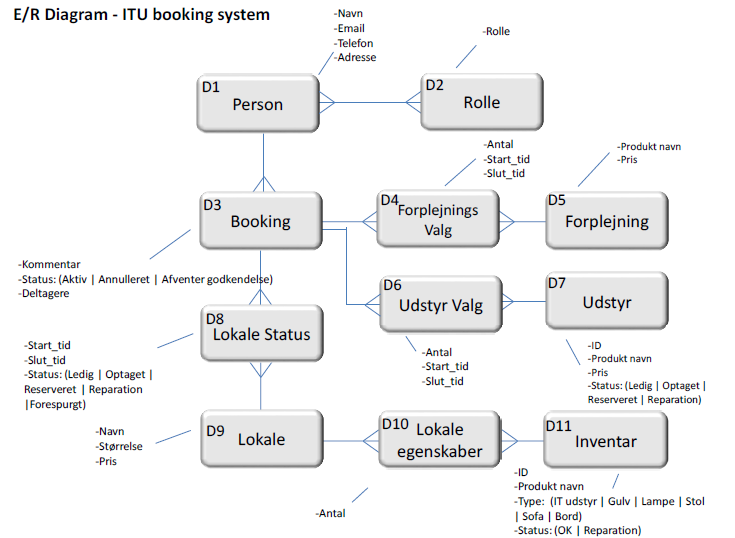
\includegraphics[width=\textwidth]{Chapters/Design/Technical/Images/KSdata}
  \caption{Kravspecifikationens datamodel}
\label{Fig:Technical_Database_ks_KSdata}
\end{figure}

Der er en række ting, som skal ændres ved datamodellen for at tilpasse den til vores løsning. 

\subsubsection{Personinformation}
\label{Technical_Database_ks_personinfo}
Det har primært været vores fokus at understøtte anvendelsen af IT-Universitetets Active Directory (AD) til at logge ind i systemet. Da ITUs AD ikke indeholder addresse

\subsubsection{Priser på lokaler/udstyr}
\label{Technical_Database_ks_prices}

\subsubsection{Lokale status}
\label{Technical_Database_ks_roomStatus}

\subsubsection{Lokale egenskaber}
\label{Technical_Database_ks_roomProperties}

\subsubsection{Inventar- og udstyrstyper}
\label{Technical_Database_ks_types}

\subsubsection{Udstyr}
\label{Technical_Database_ks_eChoice}

\subsubsection{Forplejning}
\label{Technical_Database_ks_catering}

\subsection{Vores datamodel}
\label{Technical_Database_our}

Kravspecifikationens kapitel \textit{D} \cite[s.14]{kravspec} præsenterer følgende model for det data, systemet skal bruge:
\begin{figure}[h!]
  \centering
    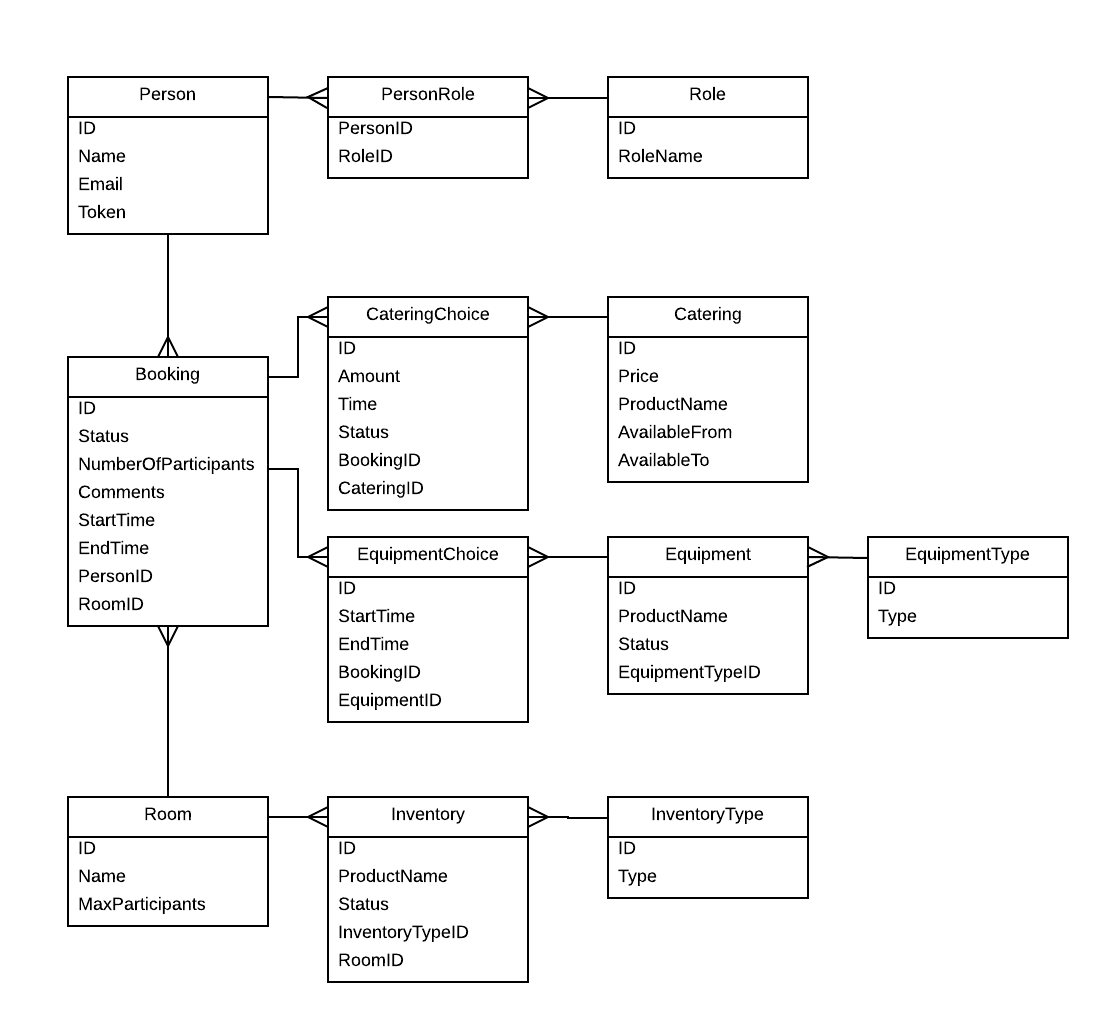
\includegraphics[width=\textwidth]{Chapters/Design/Technical/Images/OurDataModel}
  \caption{Datamodellen til vores løsning}
\label{Fig:Technical_Database_our_datamodel}
\end{figure}